\documentclass[a4paper,10pt]{article}
%\usepackage[T1]{fontenc}
\usepackage[utf8]{inputenc}
\usepackage[swedish]{babel}
\usepackage{color}
\usepackage{graphics}

\title{Webbteknik för ingenjörer \\
	Laboration 2}
\author{John-Patrik Nilsson \\
	e-mail: jpatrik.nilsson@gmail.com \\
	Skype: j-p.nilsson}
\date{}

\begin{document}

\maketitle
%\tableofcontents

\pagestyle{empty}
\thispagestyle{empty}

\section{Inledning}

Syftet med denna rapport är att beskriva innehållet och utförandet av laboration 2 som gjordes i distanskursen Webbteknik för ingenjörer våren 2009 vid Umeå Universitet.

Målsättningen med laborationen var att ge en djupare inblick i HTML, CSS och riktlinjer för användbarhet, samt att understryka värdet av att separera innehåll från utseende. Laborationsdeltagarna erhöll en bild (se figur~\ref{specifikation}) vilket fungerade som en specifikation, och de skulle därefter konstruera en webbplats utifrån denna specifikation.

Vid utförandet av laborationen användes laborationehandledningen som handledning, och som hjälpmedel vid laborationen användes en persondator med enkel textediteringsprogram samt browsern Firefox version 3.0.5. Diverse elektroniska dokument (webbsidor), samtliga listade i litteratursförteckningen, användes som hjälpdokumentation.

Sammanfattningsvis finns som bilaga i slutet av denna rapport det CSS-dokument som utgör laborationen. \\

\textbf{Keywords:} HTML, CSS, meny, laboration, WCAG, WAI.

\section{Analys av problemet}

Laborationens utförande sammanfattas bäst av dessa moment:

\begin{enumerate}
	\item Analys av specifikationen; förstå syftet med webbplatsen.
	\item Identifiera de olika delarna av webbplatsen och dess innehåll.
	\item Sortera delarna/innehållet.
	\item Bygg webbplatsen utifrån den information som inhämtats.
	\item Polera den slutgiltiga produkten; lägg till estetiska effekter.
\end{enumerate}

Vid en analys av den givna specifikationen framgick det att webbplatsen bestod av ett par bilder, en horisontell meny, samt ett eller flera block med text. Det framgick även att webbplatsen handlade om hälsa och välbefinnande. Laborationen krävde även att man vid skapandet av webbplatsen tog hänsyn till World Wide Web Consortiums (W3C) användbarhetsriktlinjer; Web Accessibility Initiative (WAI) och Web Content Accessibility Guidelines (WCAG).

\begin{figure}[h]
 \begin{center}
  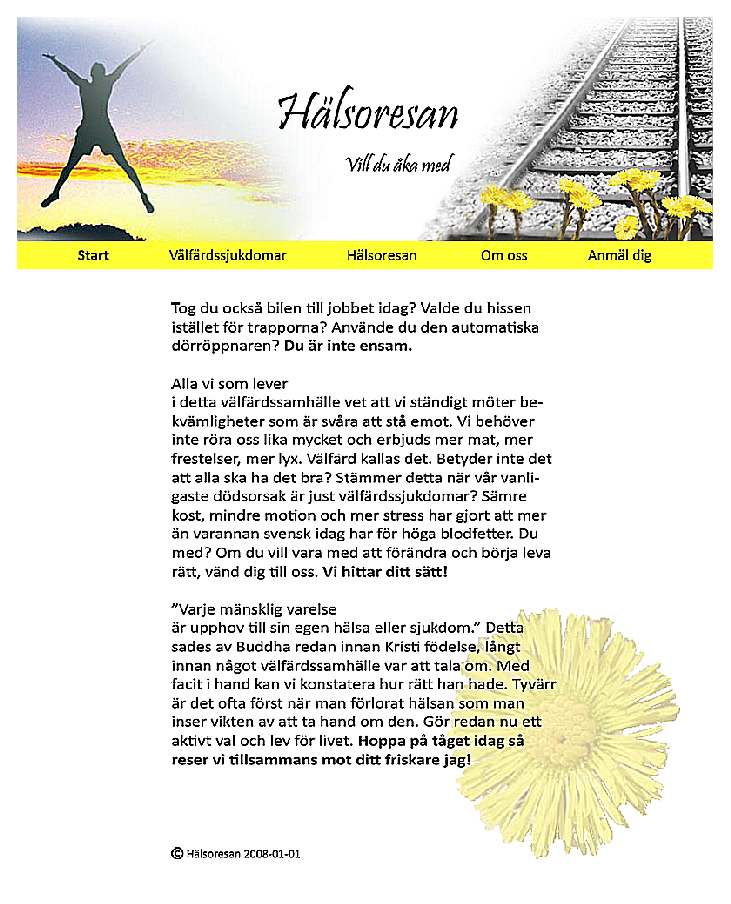
\includegraphics{specification.eps}
 \end{center}
 \caption{Bilden som fungerade som webbplatsens specifikation}
 \label{specifikation}
\end{figure}

\section{Uppbyggnad utifrån specifikation}

Då all information specifikationen var inhämtad och sorterad, var nästa steg att sätta ihop alla delar till en fungerande webbplats. Detta inleddes med att webbplatsen delades upp i fyra delar (block) så att dessa kunde innehålla de delar webbplatsen bestod av. Syftet med detta var att ge HTML-dokumentet och webbplatsen struktur, och därmed även göra det lättare att modifiera presentationen av webbplatsen med hjälp av Cascading Style Sheets (CSS). De fyra delar som webbplatsen skulle utgöras av var en header, en footer, en meny samt en innehållsdel. Var och en av dessa delar omslöts av ett div-block och gavs en unik identifikation, exempelvis \verb+<div id="menu">+.

\section{Stilmallen}

Då innehållet och strukturen på webbplatsen var på plats återstod arbetet med dess grafiska aspekt. För att lättare kunna separera utseende och innehåll på webbplatsen användes en extern CSS-stilmall vilket HTML-dokumentet länkade till i dess head-del.

Två bilder fanns med i specifikationen, och de var menade att användas till den slutgiltiga webbplatsen. Den ena bilden placerades i header-blocket, och den andra placerades som bakgrundsbild längst ner till höger i innehålls-blocket. Eftersom menyn var en lista med endast en nivå, valdes det att representera den som en horisontell inline-lista av länkar. Innehålls-blocket gavs extra padding och fylldes med icke-meningsfull latin för att representera innehållet.

\section{Polering av den grafiska presentationen}

Den grafiska representationen av webbplatsen polerades visuellt genom att det lades till diverse effekter. Den första effekten som lades till var en så kallad hover-effekt där länken i menyn som muspekaren är ovanför presenteras annorlunda än de andra länkarna i menyn. Detta gjordes för att det såg bättre ut (subjektivt) samt för att det skulle vara lättare att navigera på sidan. Därefter, med samma motivation som föregående effekt, lades ytterligare en effekt till med resultatet att man kunde se var på webbplatsen man befann sig genom att titta på menyn; den länken som hänvisade till den aktuella sidan visades på ljus bakgrund. För att öka tydligheten ännu ett steg skapades ett span-block med texten \"du är här\", som placerades under den länk som hänvisade till den aktuella sidan (se figur~\ref{meny} nedan för förtydligande). Denna typ av effekt framställs vanligtvis med hjälp av JavaScript, men man kan få liknande effekt genom att endast använda CSS, vilket demonstreras i denna laboration. Processen och CSS-kod för denna effekt förklaras i detalj nedan. \\
\\
\fbox{\parbox{12cm}{
\textsl{(Först gavs varje body element på webbplatsen en unik identitet, detta kunde åstakommas antingen genom att deklarera elementets id eller dess class. Eftersom id-identifikationen kunde användas till en CSS-signatur (Meyer, 2002) valdes det att använda class-identifikationen vid skapandet av denna webbplats.)} }}
\begin{verbatim}
    <body class="index">
\end{verbatim} 
\\
\fbox{\parbox{12cm}{
\textsl{(Nästa steg var att ge varje länk i menyn, samt själva menyn, en liknande unik identifikation.)} }}
\begin{verbatim}
    <div id="menu">
     <ul>
      <li><a class="index" href="index.html"> Index </a>
\end{verbatim} 
\\
\fbox{\parbox{12cm}{
\textsl{(I CSS-dokumentet länkades (metaforiskt) därefter de olika body-elementen ihop med respektive länk i menyn, och länkarna gavs en godtycklig grafisk representation.)} }}
\begin{verbatim}
    body.index #menu a.index {...}
\end{verbatim}

\begin{figure}[h]
 \begin{center}
  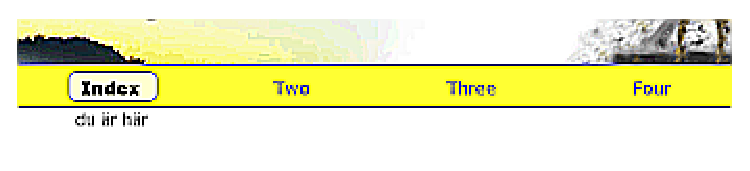
\includegraphics{menu.eps}
 \end{center}
 \caption{Menyn på webbplatsen med runda hörn}
 \label{meny}
\end{figure}

Som en avslutande försköning av webbplatsens grafiska presentation gavs diverse ramar runda hörn (se bild ovan), vilket enkelt skapades med ett par extra rader CSS-kod (till Mozilla och Safari browsers) (se CSS-kod nedan). För att runda hörn skall kunna visas i Microsofts Internet Explorer (IE) krävs det en hel del extra arbete; samtliga hörn måste representeras av bilder, vilket resulterar i att det måste skapas fyra små bilder för varje objekt med runda hörn. Stöd för runda hörn i IE ignorerades vid skapandet av webbplatsen i laborationen av två skäl; runda hörn är endast en estetisk detalj, det förändrar inte användbarheten av webbplatsen, och det andra skälet var att stöd saknades för IE på arbetsstationen som användes vid laborationen. \\
\\
\fbox{\parbox{12cm}{
\textsl{(För att få runda hörn på HTML-elementen adderades två rader CSS-kod till respektive HTML-elements stilmall. Den första raden är för att webbsidan ska visas med runda hörn med radien 8 pixlar i Mozilla-liknande browsers och den andra är för att få samma effekt med Safari-browsers.)} }}
\begin{verbatim}
    -moz-border-radius: 8px;
    -webkit-border-radius: 8px;
\end{verbatim}

\newpage

\section{Litteraturförteckning}

All information hämtad och läst under perioden Februari--Mars, 2009. \\
\\
Webb, Dan \& Griffiths, Patrick, 2003: \textsl{Suckerfish Dropdowns} (23.2.2009.)\\ 
\verb+http://www.alistapart.com/articles/dropdowns/+ \\
--- Hur man gör en dropdown-meny. \\
\\
(1.2.2009.) \verb+http://www.w3schools.com+ \\
--- Interaktiv HTML- och CSS-läroplats. \\
\\
(28.1.2009.) \verb+http://www.tfe.umu.se/courses/systemteknik/webbkurser/WU/+\\\verb+Laborationer/Laboration_xhtml_css.doc+ \\
--- Laborationshandledningen som användes. \\
\\
Meyer, Eric A., 2002: \textsl{CSS signatures} (7.3.2009.) \\ 
\verb+http://archivist.incutio.com/viewlist/css-discuss/13291+ \\
--- Om CSS-signaturer. \\
\\
Johansson, Roger: \textsl{Setting the current menu state with CSS} (7.3.2009.) \\
\verb+http://www.456bereastreet.com/archive/200503/+\\
\verb+setting_the_current_menu_state_with_css/+ \\
--- Hur man sätter aktuell status i en meny med hjälp av CSS.

\appendix

\section{Webbsidans kompletta CSS-stilmall}

\begin{verbatim}
body {
	color: black;
	background-color: white;
	font-family: verdana;
	font-size: small;

	width: 800px;
	margin: 0px auto;

	border: 1px solid #999999;
	-moz-border-radius: 8px;
	-webkit-border-radius: 8px;
}
body.index #menu a.index, 
body.two #menu a.two, 
body.three #menu a.three, 
body.four #menu a.four, 
body.five #menu a.five {
	font-weight: bold;
	border: 1px solid #999999;
	color: black;
	background-color: #ffffcf;
}
body.index span.index, 
body.two span.two, 
body.three span.three, 
body.four span.four, 
body.five span.five {
	position: absolute;
	padding-top: 2.2em;
	margin-left: -0.7em;
	color: grey;
	font-size: 90%;
	display: block;
}
/* --------------------------------------------------------- */
div#header {
	width: 800px;
	height: 258px;
	background-image:
	url('pics/banner.gif');
}
div#footer {
	padding: 0em 10em;
	color: white;
	background-color: grey;
}
/* --------------------------------------------------------- */
div#menu {
	background-color: #ffff33;
	width: 800px;
	border-top: 1px solid #999999;
	border-bottom: 1px solid #999999;
}
#menu ul {
	margin: 0;
	padding: 0.5em;
	padding-left: 4em;
}
#menu li {
	padding-left: 3em;
	padding-right: 3em;
	display: inline;
	position: relative;
}
#menu a {
	text-decoration: none;
	color: grey;
	padding: 0.1em 0.6em;
	-moz-border-radius: 6px;
	-webkit-border-radius: 6px;
	border: 1px solid #ffff33;
}
#menu a:hover {
	color: black;
	background-color: #ffffcf;
	border: 1px solid #999999;
}
/* --------------------------------------------------------- */
div#content {
	background-image:url('pics/Tussilago.gif');
	background-repeat: no-repeat;
	background-attachment: scroll;
	background-position: bottom right; 

	padding: 4em 10em;
}
/* --------------------------------------------------------- */
span {
	display: none;
}
/* --------------------------------------------------------- */
\end{verbatim}

\newpage

\section{Den färdiga webbplatsen}

\begin{figure}[h]
 \begin{center}
  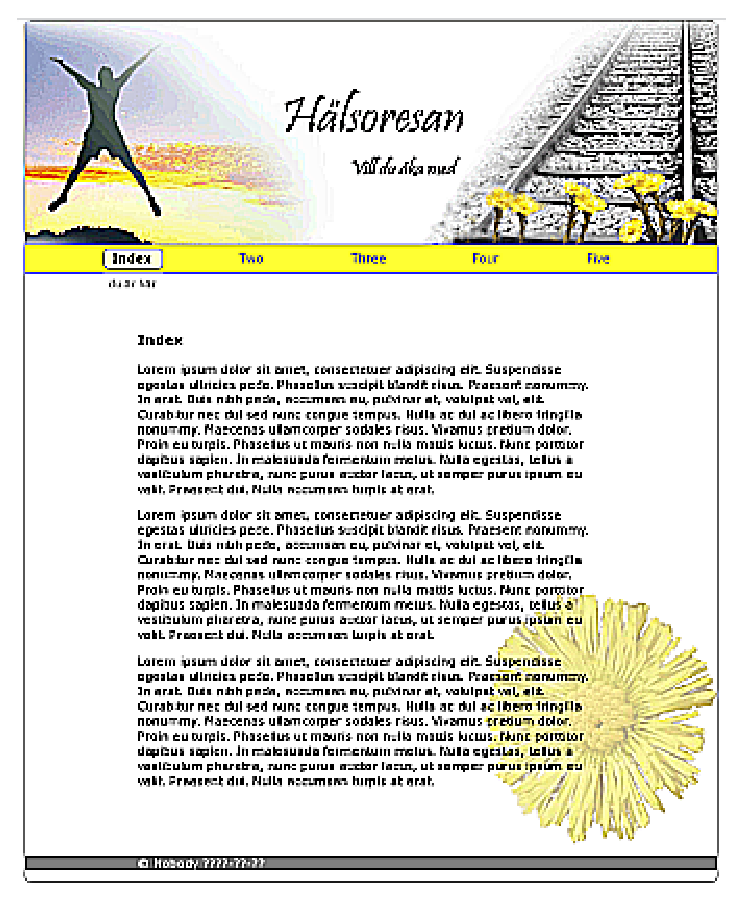
\includegraphics{complete.eps}
 \end{center}
 \caption{Bild av den färdiga webbplatsen som visad i Firefox 3.0.5}
 \label{complete}
\end{figure}


\end{document}
